\documentclass{beamer}
\usepackage{mdframed}
\usepackage{graphicx}
\usepackage{subcaption}
\usepackage{tikz}
\usepackage[french]{babel}
\usepackage[utf8]{inputenc}

\usepackage{multirow}
\usepackage{textpos}


\definecolor{TUeRed}{RGB}{170,0,0}
\definecolor{TUeBlue}{RGB}{0,68,170}
\setbeamertemplate{footline}
{
	\leavevmode%
	\hbox{%
		\begin{beamercolorbox}[wd=.5\paperwidth,ht=2.25ex,dp=1ex,leftskip=5mm]{author in head/foot}%
			\usebeamerfont{author in head/foot}\insertauthor
		\end{beamercolorbox}%

		\begin{beamercolorbox}[wd=.5\paperwidth,ht=2.25ex,dp=1ex,center]{date in head/foot}%
			\usebeamerfont{date in head/foot}\insertsection
		\end{beamercolorbox}}%
	\vskip0pt%
}
\setbeamertemplate{caption}[numbered]
\setbeamertemplate{navigation symbols}{}

\addtobeamertemplate{frametitle}{\vskip -0.5ex}{ 
	\begin{textblock*}{100mm}(.95\textwidth,-1cm) \tikz {\fill[white] (0,0) -- 
			(2cm,0) -- (2cm,1.1cm) -- (0.5cm,1.1cm) -- cycle;\node[TUeBlue] at 
			(0.8cm,0.5cm) {\normalsize\insertpagenumber};} \end{textblock*} }
		
\setbeamercolor{frametitle}{bg=TUeBlue}
\setbeamercolor{frametitle}{fg=white}



\author{Pierre Marrec}
\title{Estimer la RPE à partir de données de puissance}

\usetikzlibrary{calc, arrows.meta,
 positioning,fit,
  decorations.pathmorphing,
  decorations.pathreplacing,
   shapes.misc, fadings,
    shadows,backgrounds,
    shapes.geometric, arrows,babel}

        %Intro : L'intuition derrière le stage, l'objectif du stage, ce que j'ai compris de ce qu'on sait déjà.
        % Part 0 : Jeu de données 1 de 4 an et 1 avec plein d'athlètes mais sur ~ 2 ans
        % Part 1 : Résumé la séance -> PPR, FFT, HMM, learned Embedding depuis la séance entière |-> digression sur le puissance par état HR.
        % Part 2 : Prédiction de RPE -> Encoder - Decodeur // Lien avec le language ? Seq2Seq ? Audio/ video. Enchâssement -> état caché encoder -> décoder avec l'état caché et la séance. 


        % Expliquer le fonctionnement de HMM
        % réduire la partie PPR juste à l'oral
        % Aller plus vite sur la partie système et graphs du début
        % Regrouper les prédictions par mois /
        % - montrer le sur-entraînement
 
        % Plot des embeddings en annexe avec compet/séances

        % Expliquer qu'on se concentre sur une athlète dans la suite. 
        % Comparaison avec les LLM -> remplacer par fonctionnement rapide des NN (predictions + apprentissage) + embeddings
        % regarder la puissance moyenne par rapport à la RPE pour voir si y a des séances bizarres.
        % regarder les variations de la prédiction pour si au moins ça monte quand il faut et ça descend qui il faut.

        
        %Explication de la prédiction pas terrible : 
        % - pas assez de données
        % - le train et le test sont trop différents  -> essayer d'imputer 
        % - il y a des séances qui ont été supprimées, 
        % des séances pas notées,
        %  la RPE suffisamment fiable  - > Essayer avec la HR ?
\begin{document}

\begin{frame}
    \maketitle
\end{frame}
\begin{frame}
\frametitle{Système de l'athlète (seconde)}
\begin{figure}
    % \centering
    \vspace{-0.7cm}
    \resizebox{\textwidth}{!}{%
    \begin{tikzpicture}[node distance=1cm, scale=0.5, every node/.style={scale=0.7}]
        % Define color gradient
        
        % Nodes

        \visible<1-8>{ \node[draw,rectangle,fill=red!70, minimum width=4cm,align=center, minimum height=4cm] (system) {\LARGE Athlète(t) \\~\\ (Musculaire,\\Cardiovasculaire,\\neuromusculaire...)};}
        \visible<3-8>{ 
            \node[draw,rectangle, above left =-0.3cm and 1cm of system,align = center,minimum width=2.5cm,minimum height=1.5cm] (env) {Environnement};
            \node[draw,rectangle, left= 1cm of system, minimum width=2.5cm,minimum height=1.5cm] (energie) {Energie};
            \node[draw,rectangle, below left= -0.3cm and 1cm of system, minimum width=2.5cm,minimum height=1.5cm] (o2) {Oxygène};
            \draw[->] (env) -- (system);
            \draw[->] (energie) -- (system);
            \draw[->] (o2) -- (system);
            }

        \visible<2-8>{
            \node[draw,fill=yellow!50,rectangle, above =0.5cm  of system, minimum size=1.2cm] (neuro) {Activation neuromusculaire};
            \draw[->] (neuro) -- (system);
        }
        \visible<4-8>{
            \node[draw,fill=green,align=center,rectangle, right= 1.5cm of system, minimum size=1.2cm] (output) {Contraction musculaire:\\Puissance(t),\\Vitesse(t),\\Distance(t),\\ ...};
        }
        \visible<4>{
            \draw[->] (system) -- (output);
        }
        \visible<5-8>{ 
            \begin{scope}
                \shade[left color=red, right color=green!50, opacity=0.7]
                (system.east |- system.north) -- 
                (system.east |- system.south) -- 
                (output.west |- output.center) -- 
                cycle;
                \node[opacity=1,right = 1.4cm of system.center,align = center, sloped,text =black,text width = 1.5cm] {\tiny Efficacité de la transmission};
            \end{scope}
        }
        \visible<6-8>{
            \node[draw,circle,dotted,fill=white,below right= 0.6cm  and 0.05cm of system.west]  (sys-vo2max) {};
            \node[draw,circle,dotted,below =0.4cm of o2,align = center, sloped,text =black,text width = 1.5cm] (vo2) {\small VO2Max};

            \node[draw,circle,dotted,right=0.5cm of neuro,align = center, sloped,text =black] (eff) {\small Efficacité\\musculaire};
            \node[draw,circle,dotted,fill=white]  (sys-en) at (system.east) {};
            \draw[->,dotted,opacity=1]  (sys-en) -- (eff);
            \draw[->,dotted,opacity=1]  (sys-vo2max) -- (vo2);
        }
        \visible<7-8>{
            \node[draw,circle,fill=orange, below left=0.7cm and -.3cm of system, minimum size=1.2cm] (hr) {HR(t)};
            \node[draw,circle,fill=orange, below right=0.7cm and -0.3cm of system, minimum size=1.2cm] (rpe) {RPE(t)};
            \node[draw,circle,fill=orange, below =0.7cm of system, minimum size=1.2cm] (lt) {Lactate(t)};

            \node[draw,circle,dashed,fill=red!50,above  left= 0.2 and 0.5cm of system.south] (sys-hr) {};
            \node[draw,circle,dashed,fill=red!50,above right = 0.2 and 0.4cm of system.south] (sys-rpe) {};
            \node[draw,circle,dashed,fill=red!50,above= 0.2cm of system.south] (sys-lt) {};

            \draw[->,dashed]  (sys-hr) -- (hr);
            \draw[->,dashed]  (sys-rpe) --(rpe);
            \draw[->,dashed] (sys-lt) -- (lt);
        }
        \visible<8>{
        \node[below = 0.6cm of rpe] (measure) {Mesures de l'état du système ie Charge interne};
        \node[draw,rectangle,color = green,dashed,below = 1cm of output,minimum size = 2cm] (externe) {\textcolor{black}{Charge Externe}};
        \draw[->] (output) -> (externe);
        \draw[dashed,color = orange] ($(hr.north west)+(-0.4,0.4)$) rectangle ($(rpe.south east)+(0.5,-1.3)$);
        \node[draw,color = orange,dashed,left=0.1cm of measure] {  };
        }
        
    \end{tikzpicture}
    }
\end{figure}
% time frame secondes. L'état se réduit en séance puis remonte avec la récupération et on espère plus haut. 
% Ce qui nous intéresse c'est plus l'état moyen / jour. Est-ce qu'on surcompense et pas forcément les fluctuations de la journée.

% Comprendre le système est compliqué donc en général, on fixe un "niveau d'intensité" et on regarde comme la sortie du système.
% Par exemple, effort maximal. A partir de ça, on peut faire des pourcentages de l'effort maximal et voir la réponse du système.
% Transition avec le schéma d'après.
\end{frame}


\begin{frame}{Une autre manière de voir le système (journalière)}
    \begin{figure}
   \centering
   \begin{tikzpicture}[
    box/.style={draw, rectangle, minimum width=3cm, minimum height=2cm, align=center},
    arrow/.style={->, >=latex, thick},
    area/.style={draw=none, rectangle, minimum width=3cm, minimum height=5cm},
    node distance=.8cm,
    scale = 1,
    every node/.style={scale=0.7}
    ]
   % Title
%    \node[font=\large\bfseries] at (-2,3) {Planning};
   \visible<1-5>{
    \node[area] (area1) at (0,-0.5) {};
    \node[area, right=of area1] (area2) {};
    \node[area, right=of area2] (area3) {};
    \node[area, right=of area3] (area4) {};
    \node[box,fill=red!80] (athlete) at (area2) {Athlète};
    \node[below=0.5cm of area2] {Système};
   }
   \visible<2-5>{
    \node[below=0.5cm of area1] {Contraintes d'une séance};
    \draw[dotted] ($(area1.north east)+(.4,1)$) -- ($(area1.south east)+(.4,-1)$);
    \node[box,fill=green!80] (external) at (area1) {Charge externe};
    \draw[arrow] (external) -- (athlete);
   }
   \visible<3-5>{
    \node[below=0.5cm of area3] {Changement d'état};
    \draw[dotted] ($(area2.north east)+(.4,1)$) -- ($(area2.south east)+(.4,-1)$);
    \node[box,fill=orange!80] (reponse) at (area3) {Réponse};
    \draw[arrow] (athlete) -- (reponse);
   }
   \visible<4-5>{
    \draw[arrow, rounded corners=2cm]
     (reponse.north east) to[in=105,out=45]
     node[above, midway] {adaptation} (athlete.north);
    }
    \visible<5>{

        \node[below=0.5cm of area4] {Mesures de l'état};
        \draw[dotted] ($(area3.north east)+(.4,1)$) -- ($(area3.south east)+(.4,-1)$);
        \node[box,fill=cyan!80] (internal) at (area4) {Charge interne};
        \draw[arrow] (reponse) -- (internal);
    }
   % Adaptation loop  
   \end{tikzpicture}

   \end{figure}
   \end{frame}

\begin{frame}{De la seconde à la journée}
    \begin{tikzpicture}
        \tikzset{
            axis/.style={->, >=latex},
            graph/.style={thick, smooth},
            box/.style={draw, rectangle, minimum width=1.5cm, minimum height=1.25cm, align=center},
            scale = .8,
        }
        
        
        \begin{scope}[yshift=6cm,xshift=3cm]
            \draw[axis] (0,-1) -- (0,3) node[left=.5cm,rotate=90] {Puissance (W)};
            \draw (0,-1) -- (9,-1);
            \draw[dashed,->] (9,-1) -- (10,-1) node[right] {Temps (s)};
            
            \draw[graph] plot[variable=\x,domain=0:2,samples=100] 
                (\x,{1.5-0.1*\x+1*sin(30*\x r)/(1+\x) + sin(10*\x r)});
           
            % make a smooth transition to 0
            % Transition region
            \draw[graph] plot[variable=\x,domain=2:2.1,samples=100] 
            (\x,{ (1.5-0.1*2+1*sin(30*2 r)/(1+2) + sin(10*2 r)) * (2.1-\x)/0.1 
            + (0+0.01*sin(40*2.1 r)) * (\x-2)/0.1 });
    
            \draw[graph] plot[variable=\x,domain=2.1:4.1,samples=100] 
                (\x,{0.00*sin(40*\x r)});
            
            % Transition region
                \draw[graph] plot[variable=\x,domain=4.1:4.22,samples=100] 
                (\x,{ (0.00*sin(40*4.1 r)) * (4.22-\x)/0.12 
                + (2-0.1*4.22+1.5*sin(30*4.22 r)/(1+4.22) + 1.5*sin(10*4.22 r)) * (\x-4.1)/0.12 });
            
    
            
            \draw[graph] plot[variable=\x,domain=4.22:6.2,samples=100] 
            (\x,{2-0.1*\x+1.5*sin(30*\x r)/(1+\x) + 1.5*sin(10*\x r)});
    
            % Transition region
            \draw[graph] plot[variable=\x,domain=6.2:6.3,samples=100] 
            (\x,{ (2-0.1*6.2+1.5*sin(30*6.2 r)/(1+6.2) + 1.5*sin(10*6.2 r)) * (6.3 - \x)/0.1
            + 0 * (\x-6.2)/0.1 });
            % + (0.05*sin(30*6.3 r)) * (\x-6.2)/0.1 });
    
            \draw[graph] plot[variable=\x,domain=6.3:8,samples=100] 
                % (\x,{0.01*sin(30*\x r)});
                (\x,{0});
    
            \draw[graph,dashed] plot[variable=\x,domain=8:9.5,samples=100] 
                (\x,{0});
    
                \draw[decoration={brace,mirror,raise=5pt},decorate] (0,-1) -- node[below=6pt] (s1) {\small Séance} (2.1,-1);
                \draw[decoration={brace,mirror,raise=5pt},decorate] (2.11,-1) -- node[below=6pt] (r1) {\small Récupération} (4.1,-1);
                \draw[decoration={brace,mirror,raise=5pt},decorate] (4.12,-1) -- node[below=6pt] (s2) {\small Séance} (6.25,-1);
                \draw[decoration={brace,mirror,raise=5pt},decorate] (6.3,-1) -- node[below=6pt] (r2) {\small Récupération} (8,-1);
    
                \node[below =1cm of s1,box] (res1) {Résumé\\séance};
                \node[below= 1cm of s2,box] (res2) {Résumé\\séance};
                \node[below =1cm of r1] (rer1) {durée};
                \node[below =1cm of r2] (rer2) {durée};

    
                \draw[->] (r1) -- (rer1);
                \draw[->] (r2) -- (rer2);
            
                \draw[->] (s1) -- (res1);
                \draw[->] (s2) -- (res2);
    
                \node[box,below right = 1cm and -0.5cm of res1] (j1) {Jour 1};
                \node[box,below right = 1cm and -0.5cm of res2] (j2) {Jour 2};
    
                % Arrows
                \draw[->] (res1) -- (j1);
                \draw[->] (res2) -- (j2);
                \draw[->] (rer1) -- (j1);
                \draw[->] (rer2) -- (j2);
    
                \node[right= 1cm of j2] (j3) {...};
                \node[right = 1cm of j3,box] (j4) {Jour N};
    
    
    
            % \node[anchor=north east] at (10,3) {RPE: G};
            % \node[anchor=south west, text width=3cm, align=left] at (0,3) {Perception / Monse de l'athlète};
        \end{scope}
        \end{tikzpicture}    
    \end{frame}

    \begin{frame}{Les parties du stage}
       \begin{enumerate}
        \item Comprendre et nettoyer les données
        \vspace*{0.5cm} 
        \item Résumé des séances : Modèle de markov caché (MMC).
        \vspace*{0.5cm}
        \item Prédiction de la RPE : Utilisation de l'encodeur-décodeur pour prédire la RPE à partir des résumés de séance.
       \end{enumerate}
    \end{frame}

\begin{frame}{Les données }
    \begin{enumerate}
        \item 1 cycliste de juin 2020 à avril 2024\\
        Nettoyage : 
    \begin{itemize}
        \item suppression des séquences sans données $>$ 5min,
        \item interpolation au maximum, 
        \item suppression des valeurs aberrantes et interpolation,
        \item séance trop courtes ($<$ 10 min),
        \item séances avec des moyennes absurdes (négatives,trop basses).
    
    \end{itemize}
    \begin{table}
        \centering
        \begin{tabular}{lccc}
            \hline
            \textbf{etat} & \textbf{nombre de point}s & \textbf{nombres de séances} \\
            \hline
            complète & 9440286 & 1534 \\
            nettoyée & 4239646& 715\\
            \hline
        \end{tabular}
    \end{table}
        \item 13 athlètes de juin 2020 à avril 2022  : 63M de points 13,709 séances \\
             (39M de points nettoyés, 5,292 séances nettoyées)
\end{enumerate}
\end{frame}

    \begin{frame}{Modèle de Markov Caché (MMC) à 2 États}
        \centering
        \resizebox{\textwidth}{!}{
        \begin{tikzpicture}[
            node distance = 4cm and 5cm,
            state/.style = {circle, draw, minimum size=2cm},
            obs/.style = {rectangle, draw, minimum size=1.5cm},
            arrow/.style = {->, >=stealth, thick},
            label/.style = {font=\small\itshape}
        ]
        
        % États cachés
        \node[state] (S1) {$S_1$};
        \node[state, right=of S1] (S2) {$S_2$};
        
        % Observations
        \node[obs, below=2cm of S1] (O1) {$O_1$};
        \node[obs, below left =2cm and 2cm of S2] (O2) {$O_2$};
        \node[obs, below=2cm of S2] (O3) {$O_3$};

        
        % Transitions entre états
        \draw[arrow] (S1) to[bend left=30] node[above, label] {$a_{12}$} (S2);
        \draw[arrow] (S2) to[bend left=30] node[below, label] {$a_{21}$} (S1);
        
        % Auto-transitions
        \draw[arrow, loop left] (S1) to node[left, label] {$a_{11}$} (S1);
        \draw[arrow, loop right] (S2) to node[right, label] {$a_{22}$} (S2);
        
        % Émissions
        \draw[arrow, dashed] (S1) -- node[left, label] {$b_1(O_1)$} (O1);
        \draw[arrow, dashed] (S1) to[bend right=20] node[below, midway, label] {$b_1(O_2)$} (O2);
        \draw[arrow, dashed] (S2) to[bend left = 10 ] node[right, label] {$b_2(O_2)$} (O2);
        \draw[arrow, dashed] (S2) to[bend left=10] node[below, near start, label] {$b_2(O_1)$} (O1);
        \draw[arrow, dashed] (S2) -- node[right, label] {$b_2(O_3)$} (O3);
        \draw[arrow, dashed] (S1) to[bend right = 10] node[left, label] {$b_1(O_3)$} (O3);
        % Légende
        \node[label, text width=6cm, align=left, below=0.5cm of O1] {%
            $S_i$ : États cachés\\
            $O_i$ : Observations\\
            $a_{ij}$ : Probabilités de transition\\
            $b_i(O_j)$ : Probabilités d'émission%
        };
        
        % % Exemple de séquence
        % \node[label, text width=8cm, align=left, below right=0.5cm and -3cm of O2] {%
        %     Exemple de séquence possible :\\
        %     $S_1 \rightarrow O_1 \rightarrow S_1 \rightarrow O_2 \rightarrow S_2 \rightarrow O_3 \rightarrow S_2$%
        % };
        
        \end{tikzpicture}
        }
        \end{frame}
        
\begin{frame}{Premiers résultats}
    %Refaire les graphes
    \begin{figure}
        \centering
        \includegraphics[width = \textwidth]{figures/sequence}
        \caption{Les zones décrite par le HMM pour une séance}
    \end{figure}
\end{frame}
\begin{frame}{Premiers résultats}
    \begin{figure}
        \centering
        \includegraphics[width = .9\textwidth]{figures/time_no_roll}
        \caption{Temps passé dans chaque zone au cours du temps}
        \end{figure}
\end{frame}
\begin{frame}{Normalisation glissante}
    \begin{figure}
        \centering
        \includegraphics[width = .9\textwidth]{figures/time_roll}
        \caption{Temps passé dans chaque zone au cours du temps}
        \end{figure}
\end{frame}

%Le deuxième jeu de données pour comparer un peu les progressions ? 

% \begin{frame}{Prédiction pour le language}
%     Sémantique de mot -> Sémantique du mot dans son contexte -> Représentation du language apprise.
%     Prédiction du trafic ou éléctricité ?
%     Description de la séance -> Description de la séance dans le contexte "comment elle contribue à la Prédiction de RPE" 
%         -> état caché qui décrit le passé des X derniers jours.
% \end{frame}


\begin{frame}{Réseau de Neurones}
    \centering
    \resizebox{\textwidth}{!}{
    \begin{tikzpicture}[
        node distance = 2cm and 3cm,
        box/.style = {rectangle, draw, minimum width=3cm, minimum height=2cm},
        smallbox/.style = {rectangle, draw, minimum width=2cm, minimum height=1cm},
        arrow/.style = {->, thick},
        label/.style = {font=\small\itshape},
        every text node part/.style={align=center}
    ]
    
    % Réseau de Neurones comme une Boîte Noire
    \node[box, fill=gray!20] (nn) {
                            Réseau de Neurones \\(Paramètres/Poids)};    
    % Entrée
    \node[smallbox, left=of nn] (input) {Entrée};
    
    % Sortie
    \node[smallbox, right=of nn] (output) {Sortie};
    
    % Propagation avant
    \draw[arrow, blue] (input) --(nn);% node[above, label]  %{Propagation avant} (nn);
    \draw[arrow, blue] (nn) -- (output);%node[above, label] %{Prédiction} (output);
    
    % Rétropropagation
    \draw[arrow, red, bend right=30] (output) to node[above, label] {Rétropropagation} (nn);
    
    % Mise à jour des poids
    \draw[arrow, green, -latex, loop above] (nn) to node[above, label] {Mise à jour des poids} (nn);
    
    % Étiquettes supplémentaires
    \node[below=0.5cm of input, text width=3cm, align=center, label] {Données\\ d'entraînement};
    \node[below=0.5cm of output, text width=3cm, align=center, label] {Valeurs calculées};
    \node[below=0.5cm of nn, text width=5cm, align=center, label] {Paramètres ajustables\\appris pendant l'entraînement};
    
    \end{tikzpicture}
    }
    \end{frame}
    
    % Deuxième diapositive : Réseau de Neurones Récurrent
    \begin{frame}{Réseau de Neurones Récurrent (Vue déroulée)}
    \centering
    \resizebox{\textwidth}{!}{
    \begin{tikzpicture}[
        node distance = 2cm and 2.5cm,
        rnn/.style = {circle, draw, minimum size=1.5cm},
        box/.style = {rectangle, draw, minimum width=2cm, minimum height=1cm},
        arrow/.style = {->, thick},
        label/.style = {font=\small\itshape}
    ]
    
    % Cellules RNN
    \node[rnn] (rnn1) {RNN};
    \node[rnn, right=of rnn1] (rnn2) {RNN};
    \node[rnn, right=of rnn2] (rnn3) {RNN};
    
    % Entrées
    \node[box, above=of rnn1] (x1) {$x_1$};
    \node[box, above=of rnn2] (x2) {$x_2$};
    \node[box, above=of rnn3] (x3) {$x_3$};
    
    % Sorties
    \node[box, below=of rnn1] (y1) {$y_1$};
    \node[box, below=of rnn2] (y2) {$y_2$};
    \node[box, below=of rnn3] (y3) {$y_3$};
    
    % Connexions
    \draw[arrow] (x1) -- (rnn1);
    \draw[arrow] (x2) -- (rnn2);
    \draw[arrow] (x3) -- (rnn3);
    
    \draw[arrow] (rnn1) -- (y1);
    \draw[arrow] (rnn2) -- (y2);
    \draw[arrow] (rnn3) -- (y3);
    
    \draw[arrow] (rnn1) -- (rnn2);
    \draw[arrow] (rnn2) -- (rnn3);
    \draw[arrow, dashed] ($(rnn3.east)+(0.5,0)$) -- ($(rnn3.east)+(1.5,0)$);
    
    % Étiquettes
    \node[above=0.2cm of x2, label] {Séquence d'entrée};
    \node[below=0.2cm of y2, label] {Séquence de sortie};
    \node[right=of rnn3, text width=4cm, align=left, label] {%
        Le RNN traite les séquences\\
        en appliquant les mêmes\\
        opérations de manière\\
        répétée à chaque\\
        pas de temps
        %
    };
    
    \end{tikzpicture}
    }
    \end{frame}


\begin{frame}{Encoder - Décodeur}
    \resizebox{\textwidth}{!}{
\begin{tikzpicture}[
    box/.style = {rectangle, draw, minimum width=1.5cm, minimum height=0.7cm},
    arrow/.style = {->, thick},
    node distance = 1cm,
]

% Encoder (LSTM)

\node[box] (input1) at (0,0) {$t_1$};
\node[box] (input2) [right=1.2cm of input1] {$t_2$};
\node[box] (input3) [right= 1.2cm of input2] {$\cdots$};
\node[box] (inputd-1) [right= 1.2cm of input3] {$t_{d-1}$};
%embedding 
\node[box, fill=lightgray] (embedding1) [below=of input1] {Enchâssement};
\node[box, fill=lightgray] (embedding2) [below=of input2] {Enchâssement};
\node[box, fill=lightgray] (embedding3) [below=of input3] {Enchâssement};
\node[box, fill=lightgray] (embeddingd1) [below=of inputd-1] {Enchâssement};


\node[box, fill=lightgray] (lstm1) [below=of embedding1] {RNN};
\node[box, fill=lightgray] (lstm2) [below=of embedding2] {RNN};
\node[box, fill=lightgray] (lstm3) [below=of embedding3] {$\cdots$};
\node[box, fill=lightgray] (lstmd-1) [below=of embeddingd1] {RNN};

\node[color = red,left = 1cm of lstm1] (e0) {$etat_0$};

\draw[arrow] (input1) -- (embedding1);
\draw[arrow] (input2) -- (embedding2);
\draw[arrow] (input3) -- (embedding3);
\draw[arrow] (inputd-1) -- (embeddingd1);

\draw[arrow] (embedding1) -- (lstm1);
\draw[arrow] (embedding2) -- (lstm2);
\draw[arrow] (embedding3) -- (lstm3);
\draw[arrow] (embeddingd1) -- (lstmd-1);


\draw[arrow,color = red] (lstm1) -- (lstm2);
\draw[arrow,color = red] (lstm2) -- (lstm3);
\draw[arrow,color = red] (lstm3) -- (lstmd-1);
\draw[arrow,color = red] (e0) -- (lstm1);

% Decoder (ResNet)
\node[box] (inputd) [right= 4cm of inputd-1] {$t_d$};
\node[box, fill=lightgray] (embeddingd) [below=of inputd] {Enchâssement};

\node[box, fill=lightgray, minimum width=3cm] (resnet) [below=of embeddingd] {ResNet};
\node[box] (output) [below=of resnet] {RPE};

\draw[arrow] (inputd) -- (embeddingd);
\draw[arrow] (embeddingd) -- (resnet);
\draw[arrow] (resnet) -- (output);

% Connect Encoder to Decoder
\draw[arrow,color = red] (lstmd-1) -- node[below] {$etat_{d-1}$} (resnet)  ;

% Labels
% \node[above=0.5cm of input2] {Encoder Input};
% \node[above=0.5cm of inputd] {Decoder Input};
\node[below=0.5cm of output] {Predicted RPE};

% Bounding boxes
\node[fit=(input1) (input2) (input3) (inputd-1) (lstm1) (lstm2) (lstm3) (lstmd-1) (embedding1) (embeddingd1), draw, dashed, inner sep=0.3cm, label=Encodeur (LSTM)] {};
\node[fit=(inputd) (resnet) (output), draw, dashed, inner sep=0.3cm, label=Decodeur (ResNet)] {};

\end{tikzpicture}
}
\vspace*{-1cm}
\begin{itemize}
    \item 628 séquences d'entraînement de 14 séances
    \item 114 séquences de test de 14 séances
    \item L'état caché de sortie est sauvegardé pour la séquence suivante.
    \item Entrée : durée et puissance moyenne dans les 4 zones de puissance du MMC + temps entre les séances.
\end{itemize}
\end{frame}

\begin{frame}{Résultats}
    \begin{figure}
        \centering
        \includegraphics[width =\textwidth]{figures/pred/pre_full.png}
        \caption{Prédiction de la RPE pour des séquences de 14 séances}
    \end{figure}
    %create a table 
    \begin{table}
        \centering
        \begin{tabular}{lcc}
            \hline
            \textbf{Métrique} & \textbf{Train} & \textbf{Test}\\
            \hline
            Accuracy & 92,0\% & 15,6\%  \\
            Mean Absolute Percentage Error (MAPE) & 5,0\% & 45\%\\
            Weighted Average Percentage Error (WAPE) & 3,7\% & 39\% \\
            \hline
        \end{tabular}
    \end{table}
\end{frame}
\begin{frame}{Résultats : zoom}
    \begin{figure}
        \centering
        \hspace*{-1.05cm}
        \includegraphics[width =1.15\textwidth]{figures/pred/pred_2223.png}
        \caption{Prédiction de la RPE pour des séquences de 14 séances}
    \end{figure}
\end{frame}
    \begin{frame}{Résultats : différence}
    \begin{figure}
        % \centering
        \hspace*{-1.05cm}
        \includegraphics[width =1.15\textwidth]{figures/pred/diff_pred.png}
        \caption{Différence entre la prédiction et la vraie RPE}
    \end{figure}
\end{frame}

\begin{frame}{Résultats regroupés par mois}
    \begin{figure}
        \centering
        \hspace*{-1.05cm}
        \includegraphics[width = 1.15\textwidth]{figures/pred/pred_month.png} 
        \caption{Prédiction de la RPE pour des séquences de 14 séances regroupées par mois}
    \end{figure}
\end{frame}

\begin{frame}{Comprendre le réseau : espace latent}
    \begin{figure}
        \centering
        \includegraphics[width = .85\textwidth]{figures/pred/emb_train_30k.png}
        \caption{Projection des séances dans l'espace latent pour les 2 plus grandes composantes}
    \end{figure}
\end{frame}
    
\begin{frame}{Comprendre le réseau : représentation interne}
    \begin{figure}
        % \centering
        \hspace*{-1.05cm}
        \includegraphics[width = 1.15\textwidth]{figures/pred/c_time.png}
        \caption{Composantes principales de la représentation interne au cours du temps}
    \end{figure}
\end{frame}

\begin{frame}{Digression : MMC avec fréquence cardiaque}
    \begin{figure}
        \centering
        \includegraphics[width = .9\textwidth]{figures/time_hr.png}
        \caption{Temps passé dans chaque zone au cours du temps}
        \end{figure}
\end{frame}
\begin{frame}{Des résultats de progression}
    \begin{figure}
        \centering
        \begin{subfigure}{0.45\textwidth}
            \centering
            \includegraphics[width=\textwidth]{figures/4_states_roll_low.png}
            \caption{low}
        \end{subfigure}
        \begin{subfigure}{0.45\textwidth}
            \centering
            \includegraphics[width=\textwidth]{figures/4_states_roll_medium.png}
            \caption{medium}
        \end{subfigure}
        \begin{subfigure}{0.45\textwidth}
            \centering
            \includegraphics[width=\textwidth]{figures/4_states_roll_high.png}
            \caption{high}
        \end{subfigure}
        \begin{subfigure}{0.45\textwidth}
            \centering
            \includegraphics[width=\textwidth]{figures/4_states_roll_very high.png}
            \caption{very high}
        \end{subfigure}
        \caption*{Puissance moyenne par état au cours du temps avec régression linéaire}
    \end{figure}
\end{frame}

\begin{frame}{Conclusion}


    \begin{itemize}
        \item Résultats :
        \begin{enumerate}
            \item La prédiction sur le jeu d'entraînement est bon mais très mauvais sur le jeu de test. (surentraînement ?)
            \item Légere séparation des séances dans l'espace latent et tendance croissante de la réprésentation interne.
            \item Visualisation de la progression à partir d'états cachés tiré de la fréquence cardiaque.
        \end{enumerate}
        \item Limites :\begin{enumerate}
            \item Résumé de séance : pas assez représentatif ?
            \item Les données : manque des séances (nettoyée, pas trackée), le test est trop différent du training.
            \item Le modèle : pas adapté au nombre de données, pas suffisamment efficace, surentraînement
        \end{enumerate}
        \item Amélioration : 
        \begin{enumerate}
            \item MMC avec des émissions variables / effet aléatoire. Sur des fenêtres glissantes ?
            \item Apprendre une représentation implicite des séances (State Spaces Models)
            \item Utiliser des modèles de prédiction plus complexes (Convolutions temporelles, transformer, SSM)
        \end{enumerate} 
        
    \end{itemize}
\end{frame}

\begin{frame}{Profil de puissance record(PPR) de séance}
    %TODO ajouter 2 séances les graphes avec les PPR pour montrer la différence 
    % mais aussi que ça décrit pas le temps passé dans ces intensités.
    \begin{figure}
        \begin{subfigure}{0.55\textwidth}
            \centering
            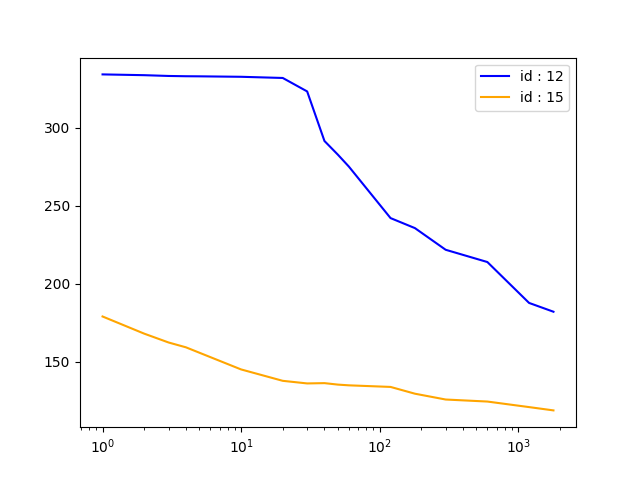
\includegraphics[width = \textwidth]{figures/comp_ppr}
        \end{subfigure}
        \begin{subfigure}{0.4\textwidth}
            \centering
            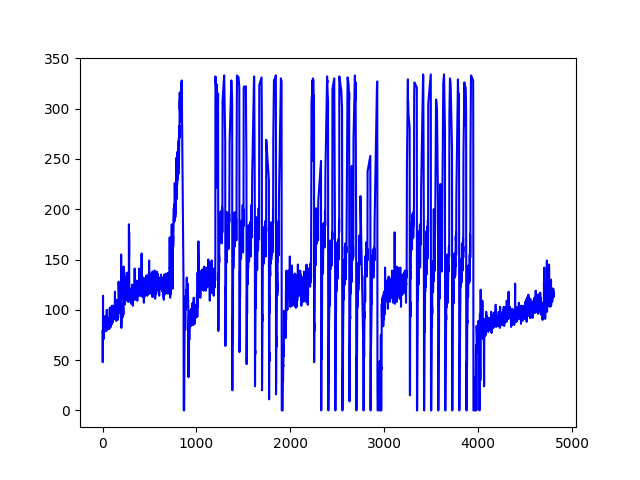
\includegraphics[height = .3\textheight]{figures/watts_12}
            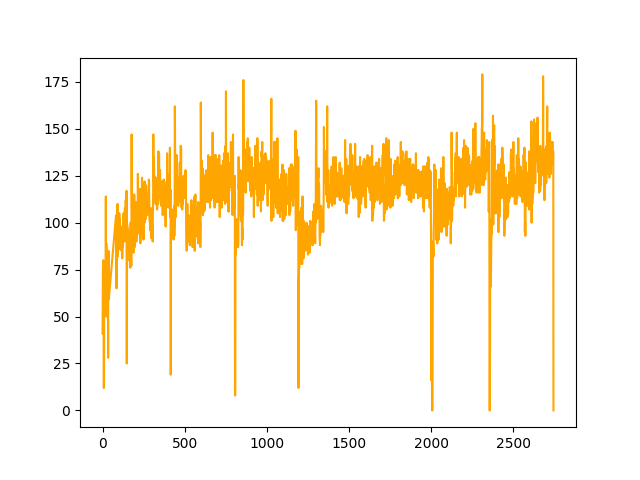
\includegraphics[height = .3\textheight]{figures/watts_15}
        \end{subfigure}
        \caption{Comparaison des PPR de deux séances}
    \end{figure}
    \vspace*{-.5cm}
    \begin{itemize}
        \item Décrit assez bien l'intensité de la séance
        \item Ne décrit pas le temps passé dans ces intensités
    \end{itemize}
\end{frame}


\begin{frame}{Les zones de PPR}
    \begin{itemize}
        \item Problème pour agréger les séances : max ou moyenne ? %TODO schéma
        \item On défini 4 zones à partir de la PPR à 30 secondes, 10 min, 1h30 \\
        $\implies$ Pas cohérent avec les zones de puissance classique et trop dépendant de la manière d'agréger.
        %Illustrations
    \end{itemize}
    \end{frame}

\begin{frame}{Matrice d'émission pour les 4 zones de puissances}
    \begin{figure}
        \centering
        \includegraphics[height=.8\textheight]{figures/mat_power.pdf}
        \caption{Matrice d'émission pour les 4 zones}
    \end{figure}
\end{frame}

\begin{frame}{Puissance moyenne par zone}
    \begin{figure}
        \centering
        \includegraphics[width = \textwidth]{figures/box_power.png}
        \caption{Box plot de la puissance moyenne par zone}
    \end{figure}
\end{frame}

\begin{frame}{Matrice de transition pour les 4 zones de FC}
    \begin{figure}
        \centering
        \includegraphics[height=.8\textheight]{figures/mat_hr.pdf}
        \caption{Matrice de transition pour les 4 zones}
    \end{figure}
\end{frame}

\begin{frame}{Fréquence cardiaque moyenne par zone}
    \begin{figure}
        \centering
        \includegraphics[width = \textwidth]{figures/box_final.png}
        \caption{Box plot de la fréquence cardiaque moyenne par zone}
    \end{figure}
\end{frame}


\begin{frame}{Large Language Model (LLM) Architecture}
    \centering
    \resizebox{\textwidth}{!}{
    \begin{tikzpicture}[
        node distance = 0.5cm,
        box/.style = {rectangle, draw, minimum width=1.5cm, minimum height=0.5cm},
        bigbox/.style = {rectangle, draw, minimum width=2cm, minimum height=1cm},
        arrow/.style = {->, thick},
        attention/.style = {->, thick, red},
    ]
    
    % Input
    \node[box] (input) at (0,0) {Entrée: "Le chat mange la souris"};
    
    % Embedding
    \node[bigbox, fill=cyan!30] (embedding) [below=of input] {Couche d'enchâssement};
    \draw[arrow] (input) -- (embedding);
    
    % Encoder
    \node[bigbox, fill=lime!30] (encoder) [below=of embedding] {Encodeur};
    \draw[arrow] (embedding) -- (encoder);
    
    % Internal Representation
    \node[bigbox, fill=yellow!30] (internal) [below=of encoder] {Representation interne};
    \draw[arrow] (encoder) -- (internal);
    
    % Attention Mechanism
    \node[bigbox, fill=orange!30] (attention) [right=of encoder] {Mechanisme d'attention};
    \draw[attention] (encoder) -- (attention);
    \draw[attention] (attention) -- (internal);
    
    % Decoder
    \node[bigbox, fill=pink!30] (decoder) [below=of internal] {Decodeur};
    \draw[arrow] (internal) -- (decoder);
    
    % Output
    \node[box] (output) [below=of decoder] {Sortie : "The cat eats the mouse"};
    \draw[arrow] (decoder) -- (output);
    
    % Annotations
    \node[left=1cm of embedding] {Vectorialisation};
    \node[left= 1cm of encoder] {Encodage contextuel};
    \node[left= 1 cm of internal] {Espace latent};
    \node[left= 1 cm of decoder] {Génération d'une séquence};
    
    % Background for the whole model
    % \begin{scope}[on background layer]
    % \node[fit=(embedding) (encoder) (internal) (attention) (decoder),
    %       draw, dashed, inner sep=0.5cm, label=right above:LLM Architecture] {};
    % \end{scope}
    
    \end{tikzpicture}
    }
    \end{frame}


\begin{frame}{Les données : 13 cyclistes}
    \begin{itemize}
        \item 13 cyclistes
        \item de juin 2020 à avril 2022 
        % \item piste, route, clm, home trainer
        % \item nettoyage : suppression des séquences sans données $>$ 5min, interpolation au maximum, suppression des séquences avec des valeurs aberrantes, séance trop courtes (négatives,trop basses, trop hautes etc.)
       \end{itemize}
       \begin{table}[ht]
        \centering
        \begin{tabular}{lcccc}
            \hline
            \textbf{Metric} & \textbf{Points} & \textbf{Nettoyé} & \textbf{Sessions} & \textbf{Nettoyé} \\
            \hline
            Mean  & 4,558,783 & 2,771,228 & 979 & 378 \\
            Std   & 1,544,788 & 1,178,575 & 292 & 163 \\
            Min   & 2,077,688 & 843,538   & 415 & 85 \\
            Max   & 8,282,392 & 5,535,237 & 1,580 & 696 \\
            \textbf{Total} & \textbf{63,822,957} & \textbf{38,797,199 }& \textbf{13,709 }& \textbf{5,292} \\
            \hline
        \end{tabular}
        \caption{Résumé des données pour les 13 cyclistes}
        \label{tab:summary_statistics}
    \end{table}
\end{frame}

\end{document}